%!Tex Root = ../main.tex
% ./Packete.tex
% ./Design.tex
% ./Deklarationen.tex
% ./Vorbereitung.tex
% ./Aufgabe1.tex
% ./Aufgabe2.tex
% ./Aufgabe3.tex
% ./Aufgabe4.tex

\section{Bonus}
\begin{frame}{Bonus}{Anzahl Formeln}
  \begin{itemize}
    \item Anzahl \alert{Zeilen in Wahrheitstabelle:} $2^{\text{\# Variablen}}$
    \item Anzahl \alert{Aussagenlogische Formeln:} $2^{\text{\#Zeilen}} = 2^{\left(2^{\text{\#Variablen}}\right)}$
    \begin{itemize}
      \item bei 3 \alert{Aussagenlogischen Variablen} gibt es $2^3=8$ Zeilen in der Wahrheitstabelle und damit $2^{(2^3)}=256$ verschiedenen Aussagenlogische Formeln, da man diese $2^3$ Zeilen auch nochmal auf \alert{exponentiell} $2^{\text{\#Zeilen}}$ viele verschiedene Arten belegen kann
    \end{itemize}
  \end{itemize}
  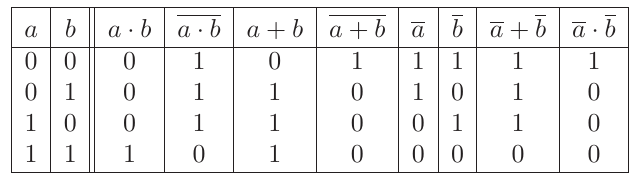
\includegraphics[width=0.5\textwidth, center]{./figures/_2021-11-22-18-46-04.png}
\end{frame}

\begin{frame}{Bonus}{Minterme und Maxterme}
  \begin{itemize}
    \item $16$ mögliche \alert{Logikfunktionen} für $2$ \alert{Aussagenlosche Variablen}
      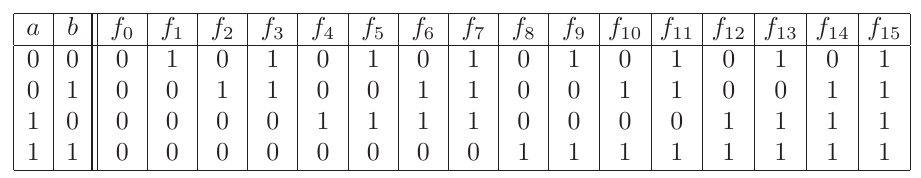
\includegraphics[width=\linewidth]{figures/_2021-11-22-18-01-18.png}
    \item $f1$, $f2$, $f4$ und $f8$ sind \alert{Minterme} (für genau eine Variation der Eingabewerte den Wert $1$)
    \item $f7$, $f11$, $f13$ und $f14$ sind \alert{Maxterme} (für genau eine Variation der Eingabewerte den Wert $0$)
  \end{itemize}
\end{frame}

\begin{frame}{Bonus}{Minterme und Maxterme}
  \begin{itemize}
    \item die $4$ \alert{Minterme} können als \alert{Konjunktionen} dargestellt werden:
      $m_{0}(a, b)=\bar{a} \cdot \bar{b}, m_{1}(a, b)=\bar{a} \cdot b, m_{2}(a, b)=a \cdot \bar{b}, m_{3}(a, b)=a \cdot b$
    \item die $4$ \alert{Maxterme} können als \alert{Disjunktionen} dargestellt werden:
      $M_{0}(a, b)=\bar{a} + \bar{b}, M_{1}(a, b)=\bar{a} + b, M_{2}(a, b)=a + \bar{b}, M_{3}(a, b)=a + b$
    \item \alert{Vergleich:}
      \[
        \begin{array}{|c|c||c|c|}
        \hline a & b & \neg a \cdot b & a + \neg b\\
        \hline 0 & 0 & 0 & 1\\
        0 & 1 & 1 & 0 \\
        1 & 0 & 0 & 1 \\
        1 & 1 & 0 & 1 \\
        \hline
        \end{array}
      \]
    \item $\neg(\neg a \wedge b) = a \vee \neg b$: \enquote{alles außer} $\neg a \wedge b$ ist $1$ $\rightarrow$ ($a=0, b=1$) ist als einziges $0$
  \end{itemize}
\end{frame}

\begin{frame}{Bonus}{Konjunktive und Disjunktive Normalform}
  \begin{itemize}
    \item aus drei \alert{Basistypen} (Disjunktion, Konjunktion oder Negation) lassen sich alle anderen \alert{Logikfunktion} erzeugen
    \item Jede Logikfunktion $f: \mathbb{B}^{2} \rightarrow \mathbb{B}$ lässt sich in \alert{Disjunktiver Normalform (DNF)}:
    $f(a, b)=f(0,0) \cdot \bar{a} \cdot \bar{b}+f(0,1) \cdot \bar{a} \cdot b+f(1,0) \cdot a \cdot \bar{b}+f(1,1) \cdot a \cdot b$
    \item als auch in \alert{konjunktiver Normalform (KNF)} darstellen:
    $f(a, b)=(f(0,0)+a+b) \cdot(f(0,1)+a+\bar{b}) \cdot(f(1,0)+\bar{a}+b) \cdot(f(1,1)+\bar{a}+\bar{b})$
    \item man möchte \alert{Logische Funktion} (Wertetabelle) mit möglichst wenig Schaltelementen realisieren $\rightarrow$ schauen, ob \alert{DNF} oder \alert{KNF} kürzer ist, je nachdem, ob die Logische Funktion (Menge an Formeln) mehr oder weniger \alert{Modelle} besitzt, also mehr oder weniger Variationen aus Aussagenlogischen Variablen besitzt, die $1$ ergeben
  \end{itemize}
\end{frame}

\begin{frame}{Bonus}{Konjunktive und Disjunktive Normalform}
  \begin{figure}
    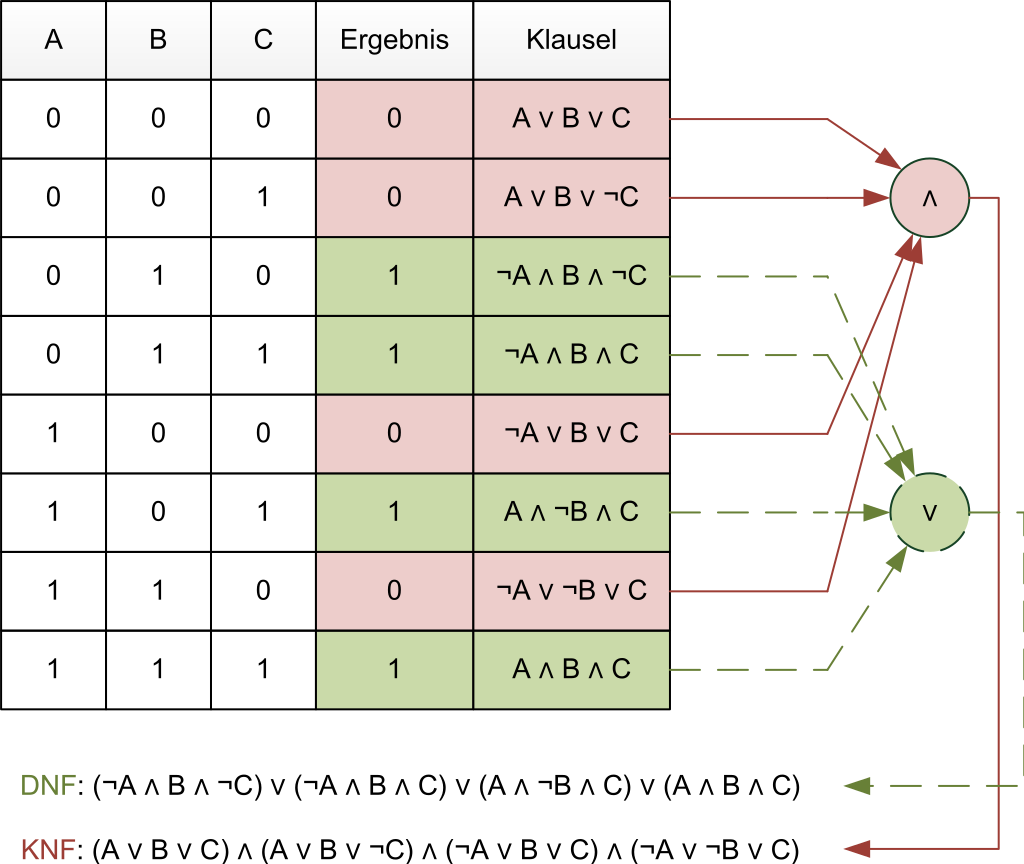
\includegraphics[height=0.6\textheight, center]{./figures/knf_dnf.png}
    \caption{Disjunktive und Konjunktive Normalform \cite{noauthor_disjunktive_2023}}
  \end{figure}
\end{frame}

\begin{frame}{Bonus}{Konjunktive und Disjunktive Normalform}
  \begin{itemize}
    \item \alert{Beispiel:} \enquote{\alert{höchstens} 2 wahre aussagenlogische Variablen}
    \begin{itemize}
      \item \alert{DNF:} $(\neg a\cdot \neg b\cdot \neg c)+(\neg a\cdot \neg b\cdot c)+(\neg a\cdot b\cdot \neg c)+(\neg a\cdot b\cdot c)+(a\cdot \neg b\cdot \neg c)+(a\cdot \neg b\cdot c)+(a\cdot b\cdot \neg c)$
      \item \alert{KNF:} $(\neg a+\neg b+\neg c)$
    \end{itemize}
  \end{itemize}
\end{frame}
